\section{Suppression des redondances dans les règles}\label{sec:regles}

\par Dans cette partie on va s'intéresser à un autre type de redondance : les redondances dans les bases de règles. Plus précisément, on s'est intéressé à deux formes particulières : 
%Une autre façon de supprimer des redondances est d'analyser la base de règles. Dans le cadre de ce projet nous avons étudié deux formes de redondances : 
\begin{itemize}
    \item les redondances au sein d'une seule et même règle, que l'on nommera redondances intra-règles (\ref{sec:intra-regles}) ;
    \item les redondances de règles par rapport aux autres règles, que l'on nommera redondances inter-règles (\ref{sec:inter-regles}).
\end{itemize}
Nous avons étudier ces redondances à l'aide de deux articles : \textit{Redundancy Rules Reduction in Rule-Based Knowledge Bases, Yongjie Zhang, Ansheng Deng} \cite{DBLP:conf/fskd/2015} et \textit{Theory and Algorithm for Rule Base Refinement, Hai Zhuge, Yunchuan Sun, Weiyu Guo} \cite{DBLP:conf/ieaaie/2003} ainsi qu'un document \cite{MINIREGLE} écrit pendant le stage d'un membre du groupe.
\par Puis on présentera une application s'appuyant sur Graal permettant de supprimer ces redondances (\ref{sec:conception-RAMIX}).


\subsection{Redondances intra-règles}\label{sec:intra-regles}
\par Avant d'entrer plus dans les détails on posera une règle de la forme $R = B \rightarrow H$ et on notera $R' = \linebreak frontierFreeze(R) =  (B' \rightarrow H')$ la règle $R$ où la frontière est gelée. 
\par On distingue deux formes de redondances intra-règles : les redondances au sein du corps de la règles (\ref{sec:redondances_corps}) et les redondances de la tête dans le corps et la tête de la règle (\ref{sec:redondances_tete_corps}).

\subsubsection{Redondances dans le corps de la règle}\label{sec:redondances_corps}
\par Il existe des redondances au sein du corps $B$ de la règle $R$ si et seulement si le nombre d'atomes dans le \textit{core} (\ref{def:Core}) de $B'$ est strictement inférieur au nombre d'atomes dans $B'$. 
\par Pour bien comprendre l'intérêt de supprimer ce type de redondance, on peut prendre l'exemple de la règle $R_1 = p(X) \land p(Y) \rightarrow q(X, Z)$. L'atome $p(Y)$ est redondant car il existe un homomorphisme : $h = \{ X \rightarrow X, Y \rightarrow X \} $ tel que $h(\{p(X), p(Y)\}) = \{p(X)\}$, donc il ne fait donc pas partie du \textit{core} de $B'$. La règle $R_1' = p(X) \rightarrow q(X, Z)$ est équivalente à $R_1$ et sans redondance dans le corps.
\par Comparons maintenant ces deux règles dans le cadre d'une saturation. Soit la base de faits $\mathcal{F} = \{p(a), p(b)\}$. Prenons tout d'abord la base de connaissance $\mathcal{KB}_1 = (\mathcal{F}, \{R_1\})$. Lors de la première étape de saturation, on peut trouver quatre déclencheurs : $(R_1,\{ X \rightarrow a, Y \rightarrow a\})$, $(R_1, \{ X \rightarrow a, Y \rightarrow b\})$, $(R_1, \{ X \rightarrow b, Y \rightarrow a\})$, $(R_1, \{ X \rightarrow b, Y \rightarrow b\})$. Si on sature à l'aide de l'\textit{oblivious chase} on obtiendrait la base de faits suivante $\mathcal{F}^*_A = \{p(a), p(b), q(a,Z_1), q(a,Z_2), q(b, Z_3), q(b, Z_4)\}$ dont le \textit{core} est $\{p(a), p(b), q(a,Z_1), q(b,Z_3)\}$. Si on prend maintenant la base de connaissance $\mathcal{KB}_2 = (\mathcal{F}, \{R_1'\})$, lors de la première étape de saturation, on peut trouver deux déclencheurs : $(R_1',\{ X \rightarrow a\})$, $(R_1', \{ X \rightarrow b\})$. Si on sature à l'aide de l'\textit{oblivious chase} on obtiendrait la base de faits suivantes $\mathcal{F}^{*}_B = \{p(a), p(b), q(a,Z_1), q(b,Z_2)\}$ qui est équivalente au \textit{core} de $\mathcal{F}^*_A$. 
\par Si on utilise les critères d'applicabilités du \textit{semi-oblivious chase} et du \textit{restricted chase}, ces redondances seraient évitées mais au prix d'un temps de calcul supplémentaire. D'où l'intérêt de supprimer ce type de redondance au sein des règles.


\paragraph{L'algorithme \textit{BodyRedundancyRemover} (\ref{algo:BodyRedundancyRemover})} Pour supprimer ce type de redondance dans une règle $R = B \rightarrow H$, il faut commencer par geler la frontière de la règle dans $B$ : on note cela $B'$. On veut en effet éviter que les variables communes avec la tête $H$ ne soient supprimées. Puis on calcule le \textit{core} de $B'$ afin de supprimer les atomes redondants. Enfin il ne reste plus qu'à dégeler la frontière dans $B'$ et retourner la règle sans redondance dans le corps $B' \rightarrow H$.
\newline
\setstretch{1}
\begin{algorithm}[H]\label{algo:BodyRedundancyRemover}
\caption{BodyRedundancyRemover}
\SetAlgoLined
\DontPrintSemicolon
\SetAlgoLined
\DontPrintSemicolon
\SetKwInOut{Input}{entrée}
\SetKwInOut{Output}{sortie}
\Input{une règle $R = B \rightarrow H$}
\Output{la règle $R$ sans redondance dans le corps}
% suppression dans le coprs -> freeze du corps -> Core -> defreeze
        $B' \gets Core(frontierFreeze(B))$ \;
        $B' \gets unFreeze(B')$ \;
        \Return $B' \rightarrow H$ \;
\end{algorithm}


% \begin{example}
%     Soit une règle $r = p(X,Y) \land p(X,b) \rightarrow p(Z,X)$. L'atome $p(X,Y)$ est redondant car il existe un homomorphisme $h = \{(X \mapsto X), (Y \mapsto b)\}$ tel que $h(p(X,Y)) = p(X,b)$.
% \end{example}

\par Une fois cette redondance supprimée dans la règle, on peut essayer de supprimer les redondances suivantes.  

\subsubsection{Redondances de la tête dans le corps et la tête de la règle}\label{sec:redondances_tete_corps}

\par Dans cette partie on prendra $B'$ le corps $B$ d'une règle où tous les atomes sont gelés. La frontière est donc aussi gelée.
\par Il existe des redondances de la tête $H$ sur le corps $B$ et sur la tête $H$ de la règle $R$ si et seulement si le nombre d'atomes dans le \textit{core} (\ref{def:Core}) de $B' \cup H$ est strictement inférieur au nombre d'atomes dans $B' \cup H$. 
\par  Pour bien comprendre l'intérêt de supprimer ce type de redondance, on peut prendre l'exemple de la règle $R_1 = p(X,Y) \rightarrow p(Y,Z) \land p(T,Z) \land p(S,T)$. Les atomes $p(T,Z)$ et $p(S,T)$ sont redondants par rapport au corps $p(X,Y)$ et une partie de la tête $p(Y,Z)$. En effet, il existe un homomorphisme : $h = \{ X \rightarrow X, Y \rightarrow Y, Z \rightarrow Z, T \rightarrow Y, S \rightarrow X \} $ tel que $h(\{p(X, Y), p(Y,Z), p(T,Z), p(S,T)\}) = \{p(X,Y), p(Y,Z)\}$, donc ils ne font donc pas partie du \textit{core} de $B' \cup H$. La règle $R_1' = p(X,Y) \rightarrow p(Y, Z)$ est équivalente à $R_1$ et sans redondance de la tête dans le corps et la tête.
\par Comparons ces deux règles dans le cadre d'une saturation. Prenons la base de connaissance $\mathcal{KB}_1 = (\mathcal{F}, \{R_1\})$ où la base de faits $\mathcal{F} = \{p(a,b)\}$. Lors de la première étape de saturation, on obtient un déclencheur : ($R_1, \{X \rightarrow a, Y \rightarrow b\}$. À l'issue de la première étape de l'\textit{oblivious chase}, on obtient la base de faits $\mathcal{F}^1_A = \{p(a,b), p(b,Z_1),\linebreak p(T_1,Z_1), p(S_1,T_1)\}$ dont le \textit{core} est $\{p(a,b),p(b,Z_1)\}$. Si on prend maintenant la base de connaissance $\mathcal{KB}_2 = (\mathcal{F}, \{R_1'\})$, lors de la première étape de saturation on trouve un déclencheur : $(R_1', \{X \rightarrow a, Y \rightarrow b\}$. Si on applique une seule étape de l'\textit{oblivious chase}, on obtient la base de faits suivante $\mathcal{F}^1_B = \{p(a,b), p(b,Z_1)\}$ qui est équivalente au \textit{core} de $\mathcal{F}^1_A$.
\par Si on utilise les critères d'applicabilités du \textit{semi-oblivious} et du \textit{restricted chase}, ces redondances ne seraient pas évitées. En effet, lors de la première étape du \textit{semi-oblivious}, la liste des déclencheurs précédemment appliqués est vide. On va donc générer tout les atomes de la tête de $R_1$. Pour le \textit{restricted chase} lors de la première étape, on ne va pas pouvoir étendre l'homomorphisme $h = (X \rightarrow a, Y \rightarrow b)$ car on produit l'atome $p(b,Z_1)$ qui n'appartient pas à $\mathcal{F} = \{p(a,b)\}$. En revanche le \textit{core} détectera ces redondances. 


\paragraph{L'algorithme \textit{HeadToBodyHeadRedundancyRemover} (\ref{algo:HeadToBodyHeadRedundancyRemover})}
va supprimer ce qui est redondant de la tête $H$ sur le corps $B$ et la tête $H$ d'une règle. Pour ce faire on va devoir construire un ensemble contenant les atomes de $B$ et de $H$ avec toutes les variables de $B$ gelées. On appellera cet ensemble $F$. Ensuite on applique le calcul du \textit{core} sur $F$ pour obtenir $F'$ sans atomes redondant. Enfin, on construit la règle $R'$ à partir de $F'$ qui sera équivalente à $R$ et sans redondance de ce type. 
\par A l'issue de cet algorithme il est possible d'obtenir une règle $R$ où la tête $H$ est totalement vide. En effet, si tous les atomes de la tête $H$ sont redondants sur le corps $B$ alors la tête sera vide car le \textit{core} supprimera tout les atomes redondant. Une telle règle sera supprimée de la base de règles $\mathcal{R}$ car elle ne produit plus aucun atome.
\newline


\setstretch{1}
\begin{algorithm}[H]\label{algo:HeadToBodyHeadRedundancyRemover}
\caption{HeadToBodyHeadRedundancyRemover} %revoir le nom
\SetAlgoLined
\DontPrintSemicolon
\SetAlgoLined
\DontPrintSemicolon
\SetKwInOut{Input}{entrées}
\SetKwInOut{Output}{sortie}
\SetKwInOut{Variables}{Variables}
\Input{une règle $R = B \rightarrow  H$}
\Output{la règle $R'$}
% suppression dans le coprs -> freeze du corps -> Core -> defreeze
    $H', F, F'\gets \{\} $ \Comment{ensembles d'atomes}
    $F \gets freeze(B, H)$ \Comment{voir notation \ref{not:freeze()}}
   
    $F' = Core(F)$\;
    \ForEach{$\alpha \in F'$} 
    {
        \uIf{$\alpha \notin B$}
        {
            $H' \gets defreeze(\{\alpha\})$\;
        }
    }
    $R' \gets (B \rightarrow H')$\;

    \Return $R'$
\end{algorithm}


\par L'application de ces deux algorithmes permettent de supprimer les redondances intra-règles étudiées. Après cette opérations pour toutes les règles d'une base de règles on va maintenant s'intéresser aux redondances entre les règles.

\subsection{Redondances inter-règles}\label{sec:inter-regles}

\par Pour un ensemble de règles, une règle va être redondante par rapport à cet ensemble si elle peut être inférée à partir des autres règles. Voici une définition un peu plus formelle d'une redondance inter-règles.

\begin{definition}
    Soit $\mathcal{R}$ une base de règle et $R \in \mathcal{R}$ une règle. On dit que $R$ est redondante dans $\mathcal{R}$ si et seulement si $\mathcal{R} \setminus\{R\} \vDash R$.
\end{definition}

\par Une des façons de savoir si une règle peut être inférée par une base de règles est d'utiliser un algorithme de chaînage avant sur la base de connaissance suivante : $\mathcal{KB} = \{B, \mathcal{R} \setminus \{R\}\} $ où $B$ est le corps de la règle $R$ à tester. Si la tête de la règle $H$ est présente dans la base de faits saturée alors on a $R$ qui est inférée par $\mathcal{R} \setminus \{R\}$. Pour detecter la présence de la tête $H$ de la règle, on peut se ramener à chercher un homomorphisme $h : H \rightarrow \mathcal{F}^*$ en ayant pris soin de geler les variables frontières. En d'autres termes, si un tel homomorphisme existe on a : $\mathcal{R} \setminus \{R\} \models R$. Donc $R$ est redondante par rapport à $\mathcal{R}$. 
\par Dans le cas contraire il y a deux possibilités. Soit l'algorithme de chaînage avant s'est arrêté, et dans ce cas, en l'absence de l'existence de l'homomorphisme $h$ décrit précédemment, on sait que $R$ n'est pas redondante par rapport à l'ensemble de règles $\mathcal{R}$. Soit l'algorithme ne s'est pas arrêté et dans ce cas on ne peut pas répondre par oui où par non. La règle $R$ est peut être redondante par rapport à l'ensemble $\mathcal{R}$ ou peut être pas.

\par Pour mieux comprendre les redondances inter-règles, on peut prendre l'exemple suivant. Soit une base de règles $\mathcal{R} = \{R_1 = p(X) \rightarrow q(X), R_2 = p(X) \rightarrow t(X), R_3 = q(X) \rightarrow t(X)\}$. On analyse règle par règle si $\mathcal{R} \setminus R$ infère $R$. Clairement $R_1$ n'est pas inférée par $\mathcal{R} \setminus R_1$ car ni $R_2$ ni $R_3$ ne produisent l'atome $q(X)$. Par contre on remarque que $R_2$ est inférée par $\mathcal{R} \setminus R_2$. On débute l'analyse avec pour base de faits $\mathcal{F}$ le corps $B$ de la règle $R_2$ : $\mathcal{F} = \{p(X)\}$. On obtient donc le déclencheur : $(R_1, \{X \rightarrow X\})$ qui va produire l'atome $q(X)$. Avec ce nouvel atome on obtient $\mathcal{F}^1 = \{p(X), q(X)\}$. Lors de la deuxième étape on obtient le délancheur : $(R_3, \{X \rightarrow X\})$ qui va produire l'atome $t(X)$ et donc $\mathcal{F}^2 =  \{p(X), q(X), t(X)\}$. La tête $H = \{t(X)\}$ de $R_2$, est incluse dans $\mathcal{F}^2$. $R_2$ peut donc être inférée à partir de $\mathcal{R}\setminus R_2$. Pour finir, on remarque que $R_3$ n'est pas redondante par rapport à $\mathcal{R} \setminus R_3$ car on obtient aucun déclencheur dès la première étape. La tête $H$ de $R_3$ n'appartient donc pas à $\mathcal{F}^*$.


\paragraph{L'algorithme \textit{interRulesRemover} (\ref{algo:SimpleRules})} va supprimer toutes les règles $R = B \rightarrow H$ redondantes par rapport à une base de règles $\mathcal{R}$. Pour chaque règle $R$ on va utiliser un algorithme de chaînage avant appliqué sur la base de connaissance suivante : $\mathcal{KB} = \{B, \mathcal{R} \setminus \{R\}\} $ où $B$ est le corps de la règle $R$ à tester. Si la tête de la règle $H$ est présente dans la base de faits saturées alors on a $\mathcal{R} \setminus \{R\} \models R$. Donc $R$ est redondante par rapport à $\mathcal{R}$. Sinon on maintient $R$ dans $\mathcal{R}$. 
\newline



\setstretch{1}
\begin{algorithm}[H]\label{algo:SimpleRules}
\caption{interRulesRemover} %revoir le nom
\SetAlgoLined
\DontPrintSemicolon
\SetAlgoLined
\DontPrintSemicolon
\SetKwInOut{Input}{entrées}
\SetKwInOut{Output}{sortie}
\SetKwInOut{Variables}{Variables}
\Input{une base de règles $\mathcal{R}$}
%\Output{la règle $R'$}
\Output{La base de règles $\mathcal{R}'$ non redondante}
% pour chaque regle on verifie si R \ r |= r
% freeze des base regle \ r et chercher un homomorphisme de r dans base regle     
    \ForEach{$R = B \rightarrow H \in \mathcal{R}$} 
    {
         $\mathcal{F} \gets$ créerFactBase($freeze$($B$)) \Comment{voir notation \ref{not:freeze()}}
         $\mathcal{F}^* \gets$ Chase($\mathcal{F}$, $\mathcal{R} \backslash \{R\}$)\;
         
         \uIf{\textit{il existe un homomorphisme }$ h : frontierFreeze(H) \rightarrow \mathcal{F}^*$}
        {
            $\mathcal{R} \gets \mathcal{R} \backslash \{r\}$\;
        }
    }
    \Return $\mathcal{R}$
\end{algorithm}



\subsection{Algorithme de suppression de redondances}\label{sec:algo-regles}

\par L'algorithme général va supprimer les redondances pour chaque règle d'une base de règles. On commencera d'abord par la suppression des redondances intra-règles en appelant les algorithmes de suppression de redondances dans le corps $B$ de la règle (\ref{algo:BodyRedundancyRemover}) suivi de la suppression des redondances de la tête sur le corps et la tête de la règles \ref{algo:HeadToBodyHeadRedundancyRemover}. Ceci sera appelée la première phase. 
\par La seconde partie de l'algorithme va supprimer les redondances inter-règles. Pour chacune des règles $R$ dans la base de règles $\mathcal{R}$ on va tester si $R$ est redondante à la base de règles $\mathcal{R} \backslash {R}$. Pour ce faire nous utiliserons l'algorithme de suppressions des redondances inter-règles (\ref{algo:SimpleRules}).

\setstretch{1}
\begin{algorithm}[H]\label{algo:redondances}
\caption{Suppression de redondances}
\SetAlgoLined
\DontPrintSemicolon
\SetAlgoLined
\DontPrintSemicolon
\SetKwInOut{Input}{entrée}
\SetKwInOut{Output}{sortie}
\Input{une base de règles $\mathcal{R}$}
\Output{la base de règles $\mathcal{R'}$}
% suppression dans le coprs -> freeze du corps -> Core -> defreeze
    $\mathcal{R}' \gets \{\}$\; 
    \ForEach{$ R = B \rightarrow  H \in \mathcal{R}$} 
    {
        $R' \gets BodyRedundancies(R)$ \;
        $R' \gets HeadToBodyAndHeadRedundancies(R')$\;
        $\mathcal{R'} \gets \mathcal{R'} \cup \{R'\}$\;
    }
    $\mathcal{R'} \gets interRulesRemover(\mathcal{R'})$\;
    \Return $\mathcal{R}'$
\end{algorithm}

On va pouvoir maintenant pouvoir passer à l'implémentation des algorithmes présentés.




\subsection{Implémentation}\label{sec:conception-RAMIX}
    \par Dans le but de pouvoir exploiter les algorithmes de suppression de redondances, nous les avons implémentés dans un nouveau \textit{package} dans GRAAL : \textit{rule\_redundancy} (figure \ref{fig:dclasse_rule_redundancy}). On présentera dans cette partie notre travail sur ces différents algorithmes de suppressions de redondances que nous proposons. Comme vu dans les sections (\ref{sec:intra-regles} et \ref{sec:inter-regles}) présentant les différents types de redondances que l'on a étudiés, on a crée deux classes, l'une traitant les redondances intra-règles et l'autre les redondances inter-règles. 
    
    \par Avant d'entrer dans les détails, présentons le format DLGP (extension \textit{.dlp}) utilisé par GRAAL pour manipuler les bases de connaissances et plus particulièrement les bases de règles. 
    
    \paragraph{Le format DLGP}
         \par Ce format est concis et facile à analyser. Cela peut être vu comme une extension du format couramment utilisé pour Datalog. Il s'appelle "dlgp" pour "Datalog Plus". Un fichier peut contenir quatre types d'éléments de connaissance : 
           \begin{itemize}
             \item les faits : $[fact_1] p(a). $
              \item les règles existentielles : $[constraint_1] ! :- X=Y, t(X,Y,b).$
              \item les contraintes négatives : $[rule_1] p(X) :- q(X).$
              \item les requêtes conjonctives : $[query_1] ? (X) :- p(X), relatedTo(X,Z), t(a,Z).$
           \end{itemize}
    
  

        \begin{figure}[!h]
        \centering
        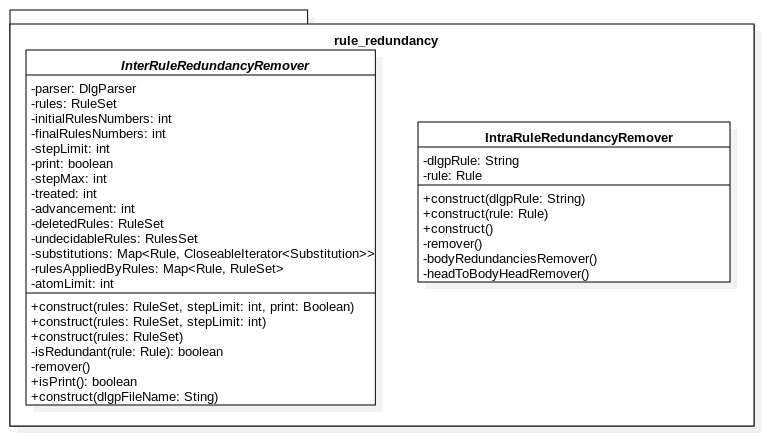
\includegraphics[width=\textwidth]{pictures/RedondanceDiagrammeClasse.png}
        \caption{Diagramme de classes du paquet graal.rule\_redundancy}
        \label{fig:dclasse_rule_redundancy}
        \end{figure}
    Maintenant que ce format a été présenté, on va aborder l'implémentation des aglorithmes.

    \paragraph{Classe IntraRuleRedundancyRemover}\ 
        \par Cette classe a pour objectif d'éliminer les redondances intra-règles (section \ref{sec:intra-regles}). On traite donc une règle. On applique dans cette classe l'algorithme \textit{BodyRedundancyRemover} (algorithme \ref{algo:BodyRedundancyRemover}) pour supprimer les redondances dans le corps et l'algorithme \textit{HeadToBodyHeadRedundancyRemover} (algorithme \ref{algo:HeadToBodyHeadRedundancyRemover}) pour supprimer les redondances de la tête sur le corps et la tête de la règle traitée. Pour effectuer le calcul du \textit{core} décrit dans l'algorithme, on utilise le \textit{core} naïf. Comme le traitement se fait sur un ensemble d'atomes issu d'une règle, il n'y a pas d'intérêt à utiliser un \textit{core} plus performant. À l'issue de ce traitement il est possible d'obtenir une règle dont la tête est vide. Cela a pour conséquence que si une telle règle est applicable, alors elle ne produira rien. On décide donc de supprimer la règle si sa tête disparaît. 
         
    \paragraph{Classe InterRuleRedundancyRemover}\ 
        \par Cette classe a pour objectif d'éliminer les redondances inter-règles (section \ref{sec:intra-regles}). Dans la méthode \textit{remover}, on applique l'algorithme \ref{algo:SimpleRules}. Cet algorithme va tester chaque règle $R$ de la base de règles $\mathcal{R}$ pour vérifier si elle est redondante par rapport à $\mathcal{R} \backslash R$. 
        \par Comme décrit dans l'algorithme on va saturer une base de faits. Cette saturation peut être infini et pourtant fournir une base de faits saturée exploitable au bout de quelques étapes permettant de décider de la redondance de la règle. Il est aussi possible qu'elle ne soit pas exploitable. On fixe donc dans tout les cas une limite d'exploration et on avant "pas à pas" dans la saturation, pour tester à chaque étape si la base de faits est exploitable. 
        \par On a crée la classe \textit{RuleApplierForRuleRedundancy} afin de récupérer chaque règle appliquées pour la saturation. Ceci permet de fournir des informations intéressante en cas de règle détectée redondante. 
        
    \paragraph{Simplifier} est un exécutable que nous avons implémenté et exécutant les algorithmes présentés précédemment. 
   % Il reprend de l'algorithme de suppressions des redondances (algorithme \ref{algo:redondances}). 
    L'exécution de ce programme se déroule en deux phases : la suppressions des redondances intra-règles et la suppressions des redondances inter-règles. 
        \par Le \textit{Simplfier} prends en paramètre une base de règle au format DLGP et retourne la base de règle dans le même format en ayant supprimé les deux types de redondances étudiés. Ce programme fournit aussi un fichier d'informations décrivant les redondances trouvées. Pour les redondances intra-règles, on précise quel est le type de la redondance : 
        \begin{itemize}
            \item corps dans le corps
            \item tête dans la tête
            \item tête dans le corps
            \item tête dans le corps et la tête.
        \end{itemize}
        Pour les redondances inter-règles, si une règle est détectée comme redondante, on précisera laquelle et quelles sont les règles qui ont été appliqués pour saturer la base de faits. 
        %Par défaut le fichier se nomme comme "infos.txt" mais il est possible de personnaliser le nom.
        \par Dans ce programme il y a trois modes. Un mode permettant d'effectuer la phase une, un autre la phase deux et le dernier pour effectuer la totalité des phases. Ce choix a été fait car pour certaines base de règles importantes, la durée du traitement de la phase une est beaucoup plus rapide (de l'ordre de quelques minutes) que la phase deux (quelques jours sur des bases de taille importante). 
        \par On peut ajouter aussi des paramètres limites. Comme expliqué dans la partie sur la classe \textit{InterRuleRedundancyRemover} qui correspond ici à la phase 2 du \textit{Simplifier}, il est possible de choisir un nombre d'étapes maximum. Il est donc possible de personnaliser ce choix en le passant en paramètre. On peut aussi fixer une limite d'atomes à ne pas dépasser pour la saturation effectué dans la phase 2. 
       
         
\subsection{Expérimentations}

\par Le \textit{Simplifier} a été testé sur différentes bases de règles. 
Certaines de ces bases sont disponibles sur le site de Graal\footnote{\url{https://graphik-team.github.io/graal/experiments1/}}. Le tableau ci-dessous décrit une partie des résultats obtenus.
\begin{center}
\begin{tabular}{|c||c|c|c|}
    \hline
    Fichier & nombre de règles initial & nombre de règles après la phase 1 & nombre de règles après la phase 2 \\
    \hline
     \hline
       A.dlp & 121 & 121 & 119    \\
     \hline
       S.dlp & 53  & 53 & 45      \\
     \hline
       U.dlp & 77  & 77 & 65      \\
     \hline
       V.dlp & 222 & 222 & 222    \\
      \hline
       G.dlp & 50764 & 50764 & calcul non terminé \\
     \hline
       exR.dlp & 12 & 7 & 5 	\\
     \hline
       Onto2.dlp & 554 & 554 & 541	\\
     \hline
\end{tabular}
\end{center}

\par Pour chacun de ces fichier \textit{.dlp} on a supprimé la redondance intra-règles (phase 1) à l'élimination des redondances inter-règles (phase 2). On voit que l'exemple \textit{exR.dlp} est intéressant car lors de la phase une on supprime déjà des règles de la base de règles. Cela veut dire que les règles avaient leurs têtes vides. L'exemple \textit{V.dlp} ne contient aucunes redondances explorées par le \textit{Simplifier}. Quant au fichier \textit{U.dlp}, il contient seulement des redondances inter-règles.  
